%\documentclass[11pt,a4paper,uplatex,dvipdfmx]{ujarticle} 		% for uplatex
\documentclass[11pt,a4j,dvipdfmx]{jarticle} 					% for platex
\input{pieces/form00_header} % pieces
\input{pieces/kakenhi7} % pieces
\input{pieces/form01_header} % pieces
\input{pieces/form02_2027_header} % pieces
\input{pieces/hook3} % pieces
%#Name: kiban_b
\input{pieces/form04_jsps_headers} % pieces
\input{pieces/form04_kiban_b_header} % pieces
% ===== Global definitions for the Kakenhi form ======================
%　基本情報
%
%------ 研究課題名  -------------------------------------------
\newcommand{\研究課題名}{大量の脆弱性・攻撃手段・パッチの依存関係を考慮した証明付き修正計画の自動生成}

%----- 研究機関名と研究代表者の氏名-----------------------
\newcommand{\研究機関名}{電気通信大学}
\newcommand{\研究代表者氏名}{田原 康之}
\newcommand{\me}{\underline{\underline{Y.~Tahara}}} 
%---- 研究期間の最終年度 ----------------
\newcommand{\研究期間の最終元号年度}{12}  %令和で、半角数字のみ
%========================================

\input{pieces/inst_general_images} % pieces
% user07_header
% ===== my favorite packages ====================================
% ここに、自分の使いたいパッケージを宣言して下さい。
\usepackage{wrapfig}
%\usepackage{amssymb}
%\usepackage{mb}
%\DeclareGraphicsRule{.tif}{png}{.png}{`convert #1 `dirname #1`/`basename #1 .tif`.png}
\usepackage{lineno}
\usepackage{multicol}
%\usepackage{ulem}
\usepackage{udline}
\usepackage{url}
\usepackage{here}
%\usepackage{amssymb}
%\usepackage{mb}
%\DeclareGraphicsRule{.tif}{png}{.png}{`convert #1 `dirname #1`/`basename #1 .tif`.png}
\usepackage{lineno}

% ===== my personal definitions ==================================
% ここに、自分のよく使う記号などを定義して下さい。
\newcommand{\klpionn}{K_L \to \pi^0 \nu \overline{\nu}}
\newcommand{\kppipnn}{K^+ \to \pi^+ \nu \overline{\nu}}

% ----- 業績リスト用 -------------
\newcommand{\paper}[6]{%
	% paper{title}{authors}{journal}{vol}{pages}{year}
	\item ``#1'', #2, #3 {\bf #4}, #5 (#6).			% お好みに合わせて変えてください。
}

\newcommand{\etal}{\textit{et al.\ }}
\newcommand{\ca}[1]{*#1}	% corresponding author;   \ca{\yukawa}  みたいにして使う
\newcommand{\invitedtalk}{招待講演}

\newcommand{\yukawa}{H.~Yukawa}					% no underline
%\newcommand{\yukawa}{\underline{\underline{H.~Yukawa}}}	% with 2 underlines
\newcommand{\tomonaga}{S.~Tomonaga}

\newcommand{\prl}{Phys.\ Rev.\ Lett.\ }		% よく使う雑誌も定義すると楽

% ===== 欄外メモ ==================
\newcommand{\memo}[1]{\marginpar{#1}}
%\renewcommand{\memo}[1]{}	% 全てのメモを表示させないようにするには、行頭の"%"を消す

\renewcommand{\baselinestretch}{.92}

\input{pieces/hook5} % pieces

\begin{document}

\setulsep{-0.1ex}

\input{pieces/hook7} % pieces
%#Split: 01_purpose_plan  
%#PieceName: p01_purpose_plan
\input{pieces/p01_purpose_plan_00}
\section{１　研究目的、研究方法など}
%　　　　＜＜最大　5ページ＞＞

%s02_purpose_plan_with_abstract
%\JSPSInstructions		% <-- 留意事項。これは消すか、コメントアウトしてください。
\noindent
\textbf{（概要）}\\
%begin 研究目的及び研究計画の概要空行付き ＝＝＝＝＝＝＝＝＝＝＝＝＝＝＝＝＝＝＝＝
近年，\ul{LLM}の高度化により，\ul{大量の脆弱性}と複数脆弱性を\ul{連鎖させる攻撃}が短時間で発見される．またLLMは脆弱性修正のための\ul{パッチの自動生成}が可能だが，\ul{信頼性が低い}ので\ul{形式検証}を用いて正しさを保証する試みもある．しかしすべてを個別に精査・修正・検証することは\ul{コスト上困難}である．本研究では (1) 脆弱性，攻撃経路，資産，パッチ，検証コスト等を統合した\ul{トリアージパッチ知識グラフ（TRKG）}を構築し，重大度，到達可能性，悪用可能性，連鎖攻撃上の役割を考慮した，根拠追跡可能な優先順位付けを実現する．さらに (2) LLMと形式検証を組み合わせ，類似脆弱性に再利用可能な\ul{証明付き修正パターン}も用いてパッチを効率的に生成する．加えて (3) パッチ間の依存・競合・包摂等の関係を推論し，すべての重大な攻撃経路を遮断する最小かつ十分な修正計画を生成する．そして (4) 以上を統合した大量脆弱性修正基盤を構築・評価し，正しさの保証と修正・検証コスト削減の両立を実現する．

\vspace*{-.5zw}	% （概要）と（本文）の間が10行程度になるよう、必要に応じて値を調整してください。	
%end 研究目的及び研究計画の概要空行付き ＝＝＝＝＝＝＝＝＝＝＝＝＝＝＝＝＝＝＝＝
\noindent
\rule{\linewidth}{1pt}\\
\noindent
\textbf{（本文）}
%begin 研究目的と研究計画	 ＝＝＝＝＝＝＝＝＝＝＝＝＝＝＝＝＝＝＝＝

\vspace*{-1.5\baselineskip}
\begin{figure}[h]
\centering
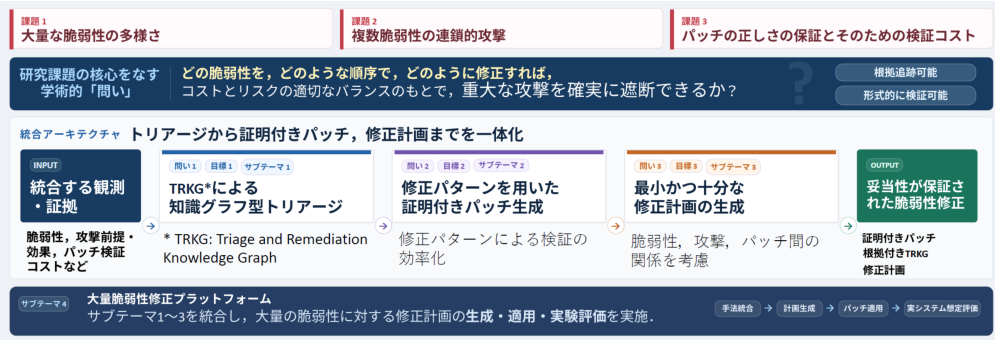
\includegraphics[width=.8\textwidth]{figs/figure}
\vspace*{-.8\baselineskip}
\caption{本研究の概要}
\label{fig:figure}
\end{figure}

\noindent\textbf{(1)本研究の学術的背景や本研究の着想に至った経緯、研究課題の核心をなす学術的「問い」}

\textbf{[背景]} 近年の\ul{大規模言語モデル（LLM）}の急速な性能向上は，利便性と引き換えに\ul{セキュリティ上の重大な問題}をもたらしつつある．たとえば最新版に近い LLM である Claude Mythos 5 は，既存のソフトウェアにおける数千件の高重大度脆弱性を，短時間で自動的に発見し，さらに攻撃コードまで作成したことが報告されている．加えて単独の脆弱性だけでなく，複数の軽微な脆弱性への\ul{連鎖的な攻撃}により，高度な権限の取得という重大なインシデントを誘発可能であることも実証された．

これに対し現状では，モデルの公開範囲を制限するという，一時的な対策が取られている．ただし理想的には，すべての脆弱性を精査し，攻撃手段を確実に遮断するための修正コード，いわゆるパッチを作成して適用することが望ましいが，コスト的に非現実的である．そこで現実的には次の各課題を考慮した上で，対策を取る必要がある．

\textbf{課題1：大量かつ多様な脆弱性} まず各脆弱性は，攻撃を受けた際の\ul{リスクの度合いの幅が大きい}．また LLM が「発見した」とされる脆弱性は，実際には到達不能，あるいは既存の防御で無害なため，修正が不要なものもある．また深刻度が高くても外部から到達困難な脆弱性より，評価上は中程度でも実際に悪用される可能性が高いものを先に修正すべき場合がある．さらにそもそも脆弱ではない箇所を誤検出することも多い．このような脆弱性の\ul{修正の要不要の判断}，および\ul{優先順位付け}を行う必要がある．

\textbf{課題2：複数脆弱性の連鎖的攻撃} 連鎖的攻撃に対しては，関係する個々の脆弱性を修正するだけでなく，一部の脆弱性の修正で連鎖を遮断できる場合や，逆に連鎖における後続の脆弱性と攻撃にも対応が必要な場合の考慮が必要である．たとえば3つの軽微な脆弱性 A，B，C があり，A と B の両方への攻撃が成功した場合に限り C への攻撃が可能となり，重大なインシデントにつながるものとする．この場合 A と B いずれか一方を修正すれば，この連鎖的攻撃を遮断できる．一方で A と B いずれか一方への攻撃の成功が前提条件である場合は，両方の修正が必要である．

\textbf{課題3：パッチの正しさの保証とそのための検証コスト} パッチは脆弱性を塞ぐだけでなく、既存機能、性能、OS や外部ライブラリなどとの互換性、および可用性を壊さないことまで要求される．またパッチが新たな脆弱性を生む可能性もある．これに対し，テストは既知の攻撃例を防げることは示せても、すべての変種や未知の経路が存在しないことまでは通常証明できない．

  なおプログラムの正しさを数学的に厳密に定義し検証する\ul{形式手法}が知られている．そして LLM と形式手法の併用により，高信頼なプログラム修正を目指した研究も進められている．しかし形式検証はテストに比べて\ul{コストがかかる}ため，大量な脆弱性への適用は非現実的である．

\textbf{[本研究の着想に至った経緯]} 応募者はこれまでに下記の各技術に関する研究成果をこれまでに挙げている：ソフトウェア工学とそのセキュリティへの応用，形式検証技術，LLM 応用技術，知識グラフ技術，およびニューロシンボリック技術．これらの研究を通じて，形式検証，LLM，および知識グラフの利用により，大量のソフトウェア脆弱性への対策を実現可能であるとの見通しを得た．このように前述の問題点の存在を認識し，各分野における研究組織の強みの活用を目指した結果，本研究の着想に至った次第である．

\textbf{[問い]} そこで本研究では，大量の脆弱性と攻撃手段に対し，LLMと形式検証によるパッチの生成において，どの脆弱性をどのような順序で修正し，また類似脆弱性に対する証明付きパッチの合成・再利用も行うことで，重大攻撃経路の遮断保証を維持しつつ，全パッチの生成・検証コストをどこまで削減できるか，という問いを立てる．そのために脆弱性の\ul{トリアージ（優先順序付け）}と，脆弱性間，攻撃手段間，およびパッチ間の\ul{関係性}も含め，判断根拠を明確にし，低コストで修正の正しさを保証することを目指す．具体的には次の各「問い」の解決を目指すものとする．

\textbf{問い1：個別の脆弱性と攻撃手段，および複数の脆弱性をまたがった連鎖的攻撃に対し，重要度，到達可能性，およびパッチの検証コストなど各種の要因を，根拠追跡可能な形でトリアージできるか}

課題1で述べたように，大量の脆弱性に対し，リスク，到達可能性，および攻撃容易性などの様々な要因がある．加えてパッチの形式検証においては，修正の規模やロジックの複雑さなどの要因により，\ul{検証コスト}にも大きな幅がある．したがってこれらの要因を適切に考慮してトリアージを行う必要がある．たとえば重大性が高く修正な脆弱性について，検証コストが低いものは修正を完全に行い，高いものは人手で修正，あるいは一部緩和策のみ実施する，などの方策が必要である．

また課題2で述べた\ul{連鎖的な攻撃}への対応については，従来のトリアージのように単に脆弱性の間の優先順位だけではなく，\ul{脆弱性間の関係}として，関わるコード間の呼び出し関係，攻撃の実行順序，あるいは攻撃による権限昇格の詳細なども考慮しなければならない．その上で適切な脆弱性の絞り込みや，修正順序も含めた修正計画の生成が必要である．

\textbf{問い2：トリアージに基づいて選定された脆弱性に対するパッチを，可能な限り正しさが保証した上で効率的に生成できるか}

課題3に関し，個別の脆弱性については，LLM と形式検証器とのフィードバックループにより，正しいパッチを作成する技術は確立されている．しかし LLM の信頼性の低さと，形式検証の計算コストの課題により，トリアージにより絞り込まれたとしても，なお大量の脆弱性を\ul{すべて修正するのは非現実的}である．そのため，たとえば複数の類似した脆弱性については，1件パッチを生成できれば，パッチの合成・再利用により，その他の脆弱性すべてについて同様に低コストで修正する，などの対応が必要である．

\textbf{問い3：複数パッチの関係性を明確にした上で，重大な攻撃を確実に遮断するために必要な修正計画を生成できるか}

さらに課題3に関連して，\ul{複数のパッチ間}には，修正計画を生成するために考慮すべき様々な\ul{関係性}がある．たとえばあるパッチを適用するには別のパッチが必要であるという依存，複数パッチを同時には適用できないという競合，あるパッチを適用すれば別のパッチが不要になるという包摂，そして1つのパッチで複数脆弱性を修正する効果の共有などがある．このような関係性を明確にした上で，問い1で確立したトリアージに基づいて修正計画を生成する必要がある．
	
\noindent\textbf{(2) 本研究の目的および学術的独自性と創造性}

\textbf{[本研究の目的]} 本研究の目的は，複数脆弱性，複数の攻撃手段，パッチの検証コスト，及び複数パッチの依存関係を考慮した修正意思決定の基礎理論を確立し，脆弱性トリアージと証明付き自動修正を統合する脆弱性修正基盤を構築することである．具体的には，以下の3つの研究目標を達成する．

\textbf{目標1：トリアージとパッチ情報を統合したオントロジーと知識グラフの構築} 問い1の解決のために，脆弱性，攻撃前提・効果，パッチの検証コスト，資産，ソフトウェア構成，観測時刻，情報源を統合するトリアージパッチオントロジーを設計し，その上で複数脆弱性及び複数パッチの依存関係を表すトリアージパッチ知識グラフ（Triage and Remediation Knowledge Graph; TRKG）を構築する．ここで知識グラフとは，概念間の関係をノードである主語と目的語，およびリンクである述語の3つ組で表したグラフであり，オントロジーとは，知識グラフの構成要素を構造的に分類し，一般的な関係性を規定することにより，知識グラフを用いた推論を可能にするものである．そして複数の脆弱性をまたがった連鎖的攻撃も考慮した上で，脆弱性間の優先順位付けとその理由の明確化を可能にする，知識グラフ型トリアージ推論を確立する．加えて知識グラフの利用により，トリアージやパッチの根拠や妥当性について，理解容易な説明を生成してユーザに提示することも可能となる．

\textbf{目標2：修正パターンを用いた効率的パッチ生成・検証} 問い2の解決のために，TRKG と，複数の類似した脆弱性を修正可能な「修正パターン」を用いて，証明付きパッチの効率的かつ高精度な生成を行う．

\textbf{目標3：修正計画生成} 問い3の解決のために，TRKG を用いて，すべての重大な攻撃経路を遮断することが検証可能な，最小かつ十分な修正計画を生成する．

\textbf{[学術的独自性]} 本研究の独自性は次の通りである．まず目標Aについては，トリアージに関する研究として文献~\cite{jiang2025vulrgmultilevelexplainablevulnerability,10.1145/3803437.3805583,11097865}があり，特に\cite{10.1145/3803437.3805583}はオントロジに基づいて，ソフトウェア部品表（Software Bill of Materials）上の複数の脆弱性に関する連鎖的攻撃を予測する．しかし当文献は部品レベルの依存関係しか考慮していない．一方で本研究は，最先端 LLM が発見するような，コードレベルでの依存関係が問題となる脆弱性への対応を目指す．

次に目標Bについては，これまでに個別の脆弱性とパッチについて，形式検証により正しさを保証する研究は多数ある．しかし複数の類似した脆弱性について，修正パターンにより一括的にパッチ生成・検証を行う研究は存在しない．

最後に目標Cについては，オントロジと知識グラフを用いて修正計画を生成する研究は存在しない．

以上により3つの研究目標それぞれについて，オントロジ，知識グラフ，および修正パターンに基づいて，大量の脆弱性に対して正しさが保証されたパッチと修正計画を，効率的に生成することを目指す点が，本研究の独自性である．

\textbf{[創造性]} 本研究の創造性は次の通りである．まずトリアージについて，個別脆弱性の重大度評価だけでなく，複数脆弱性が構成する攻撃経路上の役割も考慮して行う．次に攻撃に関する知識だけでなく，パッチの前提・順序・代替・訂正・競合まで同一の知識グラフに統合し，攻撃と修正の双方の依存関係を統一的に推論可能にする．さらに LLM によるパッチ生成を1回限りのコード生成とせず，修正パターンとその適用条件を再利用可能な知識として蓄積し，形式検証で裏付ける．
	
\noindent\textbf{(3) 関連する国内外の研究動向と本研究の位置づけ}

前述の通り本研究では，脆弱性修正に関する統一的なオントロジーに基づいて構築した TRKG に基づき，複数脆弱性に対する連鎖的攻撃も考慮したトリアージを行い，LLM と形式検証による正しさが保証されたパッチを作成し，それらの間の関係も考慮して修正計画を生成することが特徴である．一方，オントロジーと知識グラフを用いた脆弱性対策~\cite{10.1145/3803437.3805583,yadav2026cvettpkgknowledgegraph,kim2026schemaagnosticknowledgegraphconstruction,cao2026knowledgeenhancedagenticvulnerabilityrepair,mukhtar2026vulreadknowledgegraphguidedsoftwarevulnerability}，複数脆弱性にまたがる連鎖的攻撃を考慮したトリアージ~\cite{jiang2025vulrgmultilevelexplainablevulnerability,11081727,yadav2026cvettpkgknowledgegraph,11097865}，LLM と形式検証を用いたパッチの作成~\cite{cao2026knowledgeenhancedagenticvulnerabilityrepair,11081727}，および複数のパッチ間の関係の扱い~\cite{10.1109/ASE63991.2025.00087,308048,11334567}に関し，個別に扱っている研究は，それぞれ示したように存在する．一方本研究は前述した独自性により，これらの研究に対する優位性を持っていると言える．

\noindent\textbf{(4)本研究で何をどのように、どこまで明らかにしようとするのか}

本研究の各実施項目の詳細は次の通りである．

\noindent\textbf{サブテーマ1：知識グラフに基づいたトリアージ（主担当：江上，副担当：田原，清，井上）} 本サブテーマでは，目標1を達成するため，トリアージパッチ知識グラフ（TRKG）を構築し，複数の脆弱性をまたがった連鎖的攻撃も考慮した上で，脆弱性間の優先順位付けとその理由の明確化を可能にする，知識グラフ型トリアージ推論を確立する．

まず TRKG の基盤としてトリアージパッチオントロジーを開発する．そのために米国国立標準技術研究所（NIST）による Vulnerability Description Ontology (VDO) や，前述の文献などで提案されている，既存の脆弱性関連オントロジーを統合する．その上で，本研究の独自性である，形式検証と修正パターンの組み込みを可能にするためにオントロジーを拡張する．そして本オントロジーに基づき，前述の文献で提案されたものなどの既存の知識グラフを統合し，新規に発見された脆弱性と攻撃手段も取り込んで TRKG を構築する．またコードレベルの脆弱性・攻撃間関係を扱うために，コードの静的解析によりコード知識グラフを作成して TRKG に取り入れる．さらに文献~\cite{10.1145/3803437.3805583}の手法も参考にして，連鎖的攻撃も含めた脆弱性に対するトリアージ推論を確立する．

\noindent\textbf{サブテーマ2：知識グラフと修正パターンを用いた，効率的な証明付きパッチの生成（主担当：田原，副担当：石川，鄭，江上）} 本サブテーマでは，目標2を達成するため，TRKG と修正パターンを用いた，効率的な形式検証により，証明付きパッチを生成する．まず既存の脆弱性について，CWE（Common Weakness Enumeration）分類などを用いて，類似した脆弱性と修正方法を一般化し，形式検証を用いて証明付き修正パターンを生成する．次に新規の脆弱性に対し，生成済みの修正パターンの適用を試み，可能ならば適用してパッチを生成する．そうでない場合は，文献~\cite{11081727} の手法を参考にして，正しいパッチの自動生成を実現する．さらに，本脆弱性とパッチから，可能ならば新規の証明付き修正パターンを生成する．

修正パターンの例として，CWE-680 として分類されている，整数オーバーフローの発生によるバッファオーバーフロー脆弱性を挙げる．C 言語で ``（変数名） \texttt{= malloc(}（変数名） \texttt{*} （変数名）\texttt{);}''，つまり ``（変数名） \texttt{*} （変数名）''バイトのメモリを確保して左辺の変数を先頭ポインタとする，というコードがあった場合，条件次第で整数オーバーフローが起こる可能性がある．この場合，オーバーフローのチェックを行うコードを追加する，という修正を行う．

また仮にこのパターンが当初登録されていなかったとした場合，次の手順でパターンを生成できる．まずこのパターンに当てはまるパッチが複数生成されたことを前提とする．その上で，(1) パターンに当てはまるパッチ群を，類似性判定などにより特定する．(2) パッチの中の異なる部分を，前述の ``（変数名）'' のように一般化する．(3) 修正前のコードのパターンに一致する部分を全ソースコードから検索し，脆弱性の有無で分ける．(4) 脆弱性のあるものの特徴を，LLM や静的解析で特定し，パターン適用の条件とする．

\noindent\textbf{サブテーマ3：すべての重大な攻撃経路を遮断することが検証可能な，最小かつ十分な修正計画の生成（主担当：田原，副担当：清，井上，石川）} 本サブテーマでは，目標3を達成するため，パッチが生成された脆弱性に対し，全体的に整合性が保たれるようにパッチの適用を実施する修正計画を生成する．具体的には，前述した複数脆弱性に対するパッチの管理を行う研究を参考にする．その上で LLM も活用して，パッチ間の関係を統合した TRKG 上での推論と形式検証を，ニューロシンボリック技術も用いて統合することにより，正しさの保証された修正計画を生成する．

\noindent\textbf{サブテーマ4：大量脆弱性修正プラットフォームの確立（主担当：田原，副担当：清，井上，石川，鄭，江上）} 本テーマでは，まずサブテーマ1～3で確立した手法をプラットフォームとして統合し，大量の脆弱性に対する修正計画の生成・適用を可能とするプラットフォームを確立する．なおトリアージから修正計画生成までを単に直列に接続するだけでなく，必要に応じて前のタスクにフィードバックするループも組み込む．その上で実システムを想定したベンチマークを通じて実験評価を行う．

\noindent\textbf{本研究の進め方} サブテーマ1〜3については，令和 9 年度には (1) サブテーマ1については TRKG の構築を，(2) サブテーマ2については証明付きパッチ生成機構の実装を，(3) サブテーマ3については修正計画生成機構の実装を行い，令和 10 年度にはサブテーマごとに予備実験と評価・洗練を行う．サブテーマ4については，令和 9 年度にはベンチマークの選定を，令和 10 年度にはベンチマークの整備を行う．そして令和 11 年度にはサブテーマ 1〜3 で開発した手法のプラットフォームとしての統合と，ベンチマークを用いた予備実験を，令和 12 年度には最終的な実験・評価を行い，プラットフォームと評価結果を公開する．

\noindent\textbf{(5) 本研究の目的を達成するための準備状況}

「2 応募者の研究遂行能力及び研究環境」に示した研究業績を踏まえた上で，前述した参考文献を含めた関連する先行研究の調査や，必要な設備の選定などの準備を進めている．

またベンチマークとして，既存文献で用いられているものに加え，たとえばアンスロピック社が公開したリスト（\texttt{https://red.anthropic.com/2026/cvd/}）のような，実際のシステムに対して LLM により検出された多数の脆弱性として公開されたものを利用する．

\noindent\textbf{(6) 本研究がどのような国際性を有するか}

研究代表者と研究分担者はこれまでに，世界的に一流の研究者が発表の場としている海外論文誌と国際会議において，多数の業績を発表している．本研究の成果もそのような場で継続的に発表することにより，当該分野における世界の研究をけん引できるものと考える．
\begin{figure}[h]
\centering
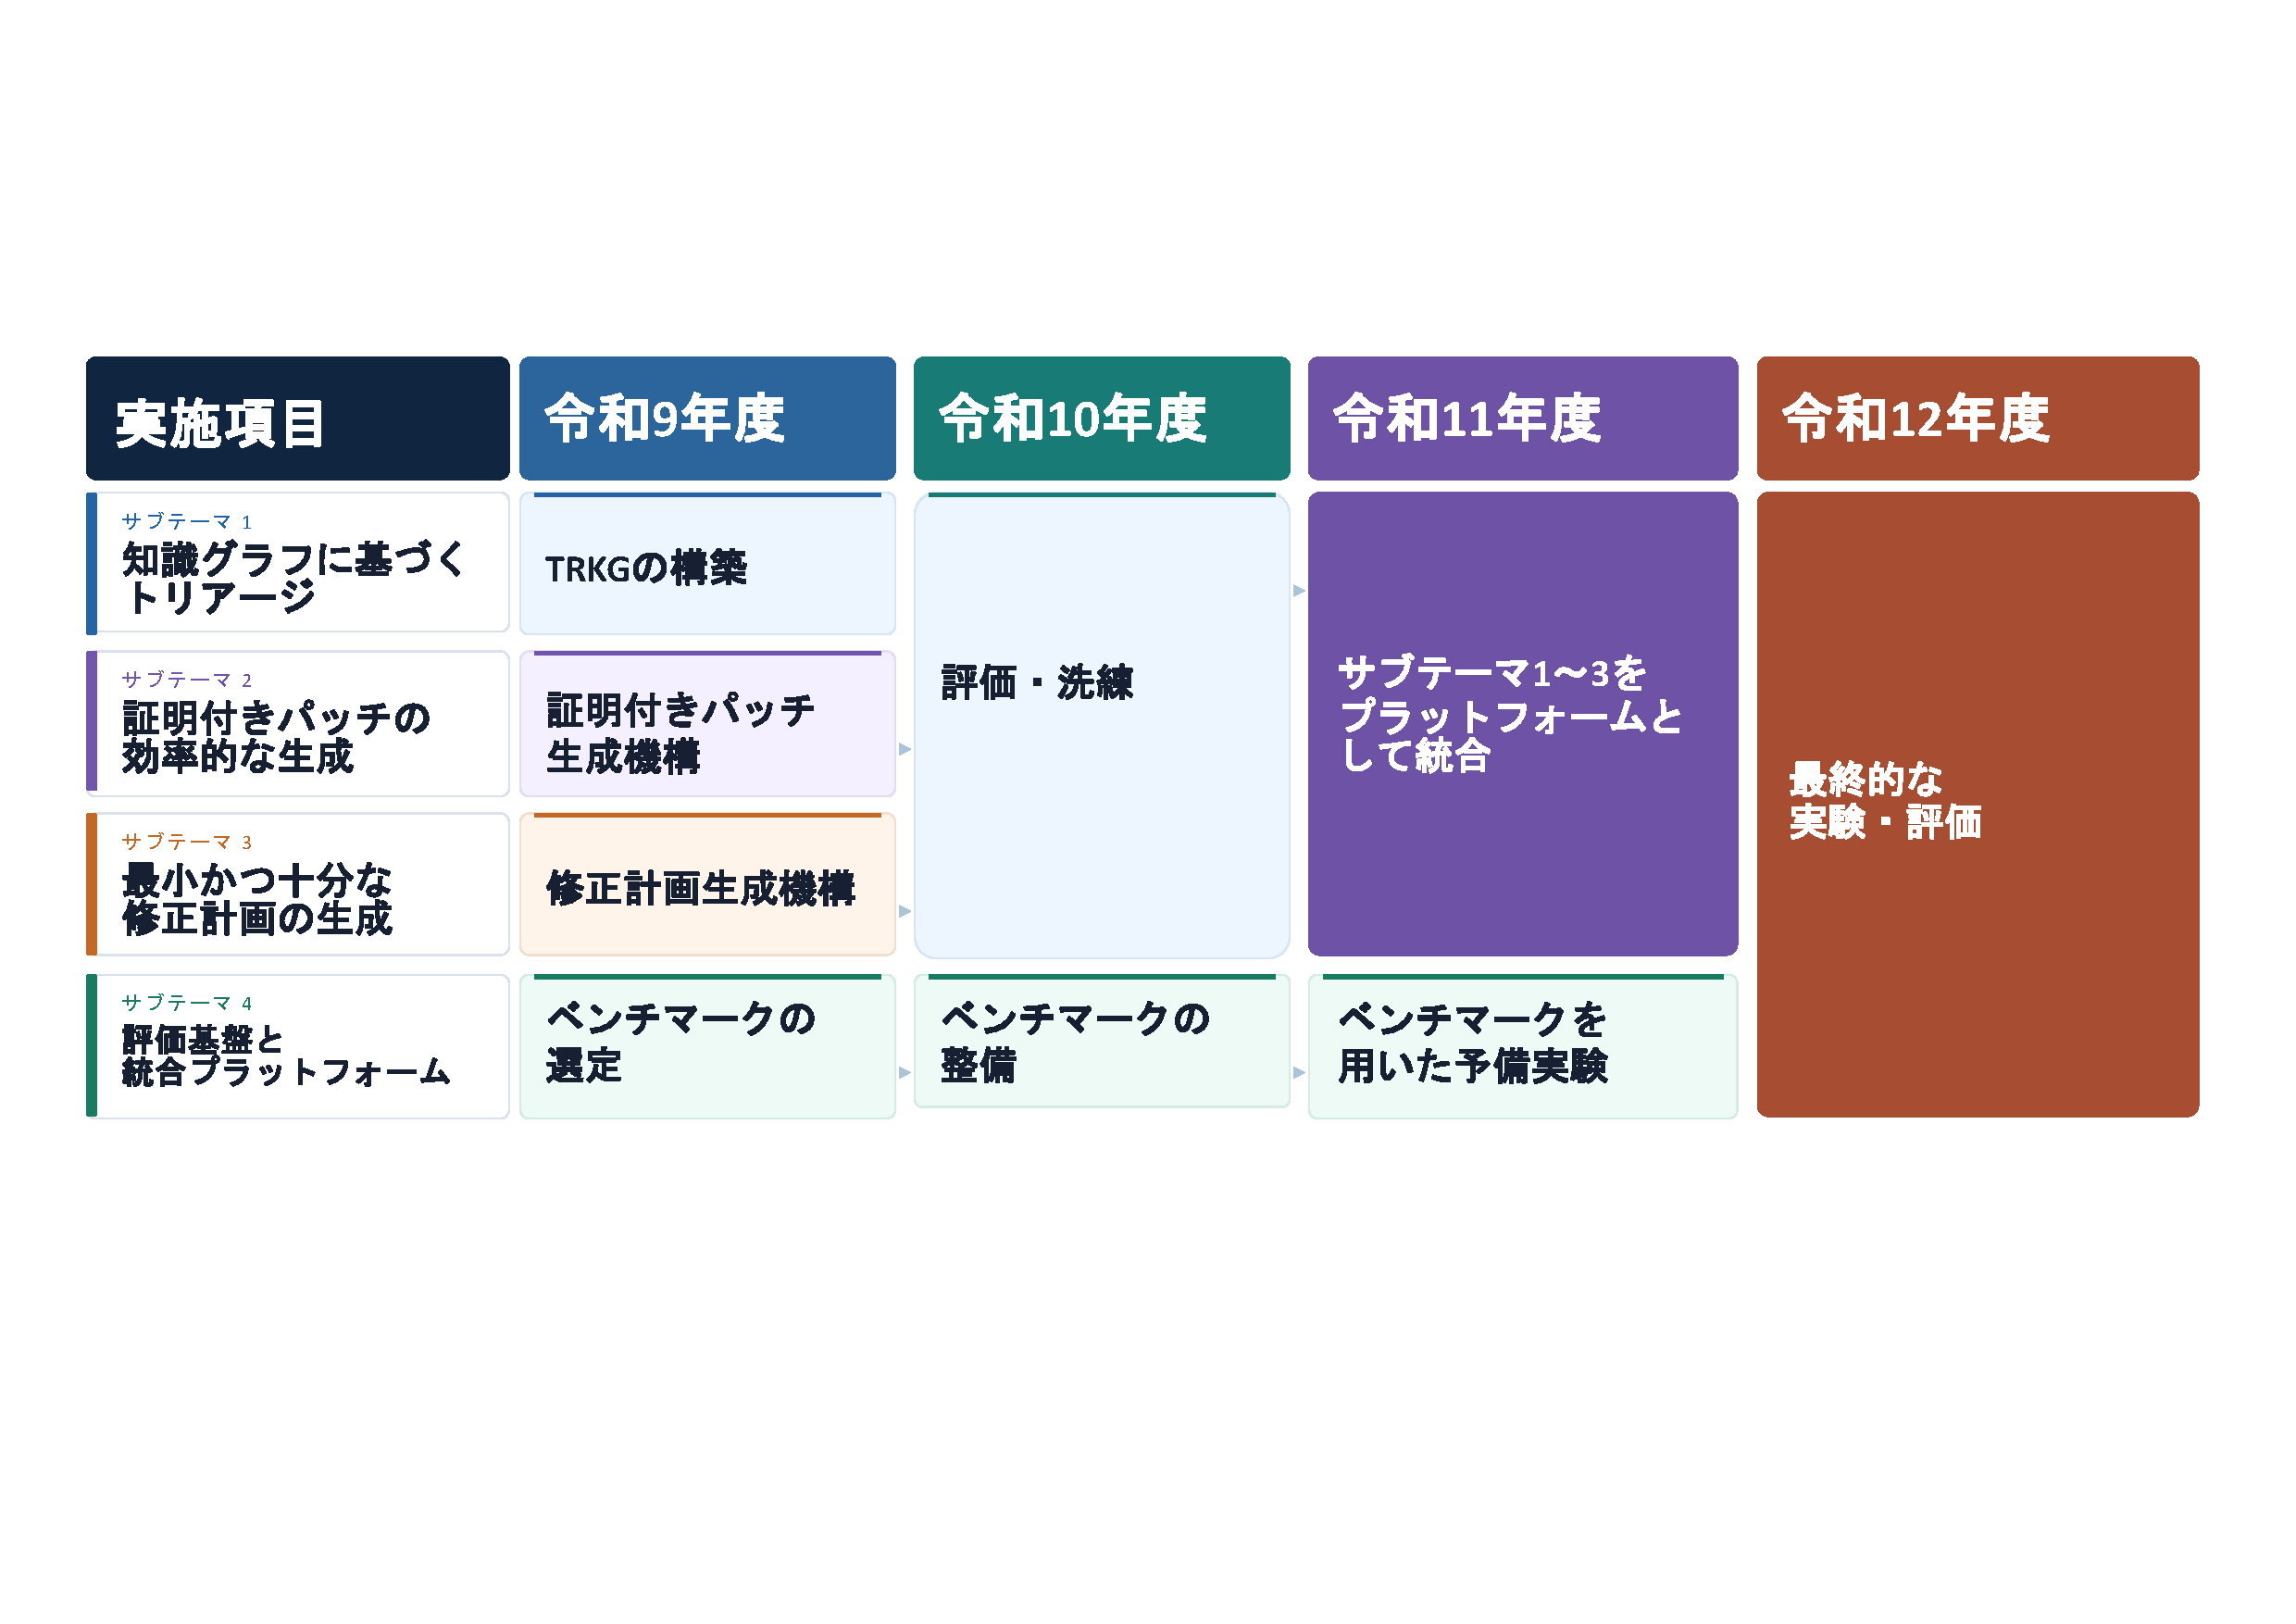
\includegraphics[width=.8\textwidth]{figs/schedule}
\vspace*{-.5\baselineskip}
\caption{本研究の進め方}
\label{fig:schedule}
\end{figure}

\noindent 参考文献：
%\vspace*{-.1\baselineskip}
\begin{enumerate}
  \setlength{\parskip}{0mm} % 段落間
  \setlength{\itemsep}{0mm} % 項目間
  \setlength{\baselineskip}{.92\baselineskip}
\bibitem{jiang2025vulrgmultilevelexplainablevulnerability}
Y.~Jiang, N.~Oo, Q.~Meng, H.~W. Lim, and B.~Sikdar.
\newblock VulRG: Multi-level explainable vulnerability patch ranking for
  complex systems using graphs, arXiv:2502.11143, 2025.

\bibitem{10.1145/3803437.3805583}
L.~Baird and A.~Moin.
\newblock Towards predicting multi-vulnerability attack chains in software
  supply chains from software bill of materials graphs.
\newblock In {\em Proc. of {FSE} 2026 Companion}, pages
  1336--1340, 2026.

\bibitem{10.1109/ASE63991.2025.00087}
Y.~Song, D.~Xie, L.~Xu, H.~Zhang, C.~Zhou, and X.~Xie.
\newblock Not every patch is an island: Llm-enhanced identification of multiple
  vulnerability patches.
\newblock In {\em Proc. of {ASE} 2025}, pages 996--1007, 2025.

\bibitem{308048}
S.~Sun, Y.~Xing, X.~Wang, S.~Wang, Q.~Li, and K.~Sun.
\newblock {DISPATCH}: Unraveling security patches from entangled code changes.
\newblock In {\em Proc. of {USENIX} Security 2025}, pages 4521--4540, 2025.

\bibitem{yadav2026cvettpkgknowledgegraph}
S.~Yadav, D.~R. Arikkat, B.~Agarwal, S.~Nicolazzo, A.~Nocera, and P.~Vinod.
\newblock CVE-TTP KG: Knowledge graph linking software vulnerabilities to
  attack behaviors, arXiv:2606.31557, 2026.

\bibitem{kim2026schemaagnosticknowledgegraphconstruction}
S.~Kim, J.~Kim, D.~Kang, D.~Kim, and I.~Lee.
\newblock Schema-agnostic knowledge graph construction via hybrid ontology
  discovery for cyber threat intelligence, arXiv:2606.01208, 2026.

\bibitem{cao2026knowledgeenhancedagenticvulnerabilityrepair}
S.~Cao, H.~Ma, L.~Yu, K.~Ding, X.~Liu, T.~Y. Zhuo, B.~Wang, X.~Lin, X.~Sun,
  L.~Wang, and D.~Lo.
\newblock Knowledge-enhanced agentic vulnerability repair, arXiv:2607.00820, 2026.

\bibitem{11334567}
O.~I. Al-Bataineh.
\newblock Interaction-aware patch assessment for multi-fault automated program
  repair.
\newblock In {\em Proc. of {ASE} 2025}, pages 3799--3803, 2025.

\bibitem{11097865}
Y.~Zhang, M.~Ward, and H.~Nguyen.
\newblock { Rethinking Attack Path Management: A New Metric for Choke Points in
  Attack Graphs }.
\newblock In {\em Proc. of {CSF} 2025}, pages 205--219, 2025.

\bibitem{mukhtar2026vulreadknowledgegraphguidedsoftwarevulnerability}
S.~Mukhtar, Y.~Yao, Z.~Sun, M.~Mustafa, Y.~S. Ong, and Y.~Sun.
\newblock VulReaD: Knowledge-graph-guided software vulnerability reasoning and
  detection, arXiv:2602.10787, 2026.

\bibitem{11081727}
N.~Tihanyi, Y.~Charalambous, R.~Jain, M.~A. Ferrag, and L.~C. Cordeiro.
\newblock { A New Era in Software Security: Towards Self-Healing Software via
  Large Language Models and Formal Verification }.
\newblock In {\em Proc. of {AST} 2025}, pages 136--147, 2025.
  % \vspace*{-.5\baselineskip}
\end{enumerate}
%end 研究目的と研究計画	 ＝＝＝＝＝＝＝＝＝＝＝＝＝＝＝＝＝＝＝＝

\input{pieces/p01_purpose_plan_01}

%#Split: 02_abilities  
%#PieceName: p02_abilities
\input{pieces/p02_abilities_00}
\section{２　応募者の研究遂行能力及び研究環境}
%　　　　＜＜最大　2ページ＞＞

% s14_abilities
%\PapersInstructions		% <-- 留意事項。これは消すか、コメントアウトしてください。
%begin 応募者の研究遂行能力及び研究環境 ＝＝＝＝＝＝＝＝＝＝＝＝＝＝＝＝＝＝＝＝

応募者はこれまでに，必要な基盤技術に関し日本で最先端の成果を挙げている．以下に，各基盤技術の詳細を示す．

\noindent \textbf{ソフトウェア工学技術：}田原，清，鄭は，ソフトウェア工学技術の分野で，重要な成果を挙げている（研究業績\ref{tahara25}, \ref{tei25}, \ref{tei24-2}, \ref{tei24-1}, \ref{tei23}, \ref{tahara17}, \ref{tahara10}）．

\noindent \textbf{形式検証技術：}田原，清，石川，鄭は形式検証技術の分野で，重要な成果を挙げている（研究業績\ref{tei23}, \ref{sei23}, \ref{sei19}, \ref{tahara17}, \ref{tahara10}）．

研究業績\ref{tei23}では，リフレクションと呼ばれる枠組みにおいて，モデル検査による検証手法を提案している．\ul{本業績はソフトウェア工学のトップジャーナルの1つである IEEE TSE}
\ul{（impact factor=6.28）に掲載され，これにより情報処理学会ソフトウェア工学研究会卓越研究賞を受賞したものである．}

\noindent \textbf{LLM 応用技術：}田原，清，鄭は，LLM 応用技術の分野で，重要な成果を挙げている（研究業績\ref{tei24-1}, \ref{tei24-3}）．

なお研究業績\ref{inoue25}, \ref{tei24-2}, \ref{tei24-1}, \ref{tei24-3}, \ref{inoue24}, \ref{inoue22-2}は，国際共同研究の結果としての成果である．

\noindent \textbf{知識グラフ技術：}江上は，知識グラフ技術の分野で，重要な成果を挙げている（研究業績）．

\noindent \textbf{ニューロシンボリック技術：}井上は，機械学習技術の分野で，重要な成果を挙げている（研究業績\ref{inoue25}, \ref{inoue24}, \ref{inoue23}, \ref{inoue22-2}）．いずれも \ul{AI や機械学習の分野の世界トップレベルのジャーナルと国際会議で発表されたものである}．

また清は、電子情報通信学会AI研究会の委員長やIEEE CS Japan Chapter幹事を務め，研究代表者として科研費・若手(A)，基盤(A)，JSTさきがけ等においてセキュリティ・プライバシと機械学習の融合領域における研究を行ってきた．筆頭著者としてIEEE論文誌に10編採録され，セキュリティトップ会議IEEE S\&P 2025 (Core rank A*)に採択されているほか，機械学習のトップ会議IJCAI (Core rank A*)のPC Boardを務めている．

このように申請者は，過去に上述の各分野で重要な業績を上げており，本研究に必要な知識と技術を持ち合わせている．

\noindent\textbf{(2) 研究環境(研究遂行に必要な研究施設・設備・研究資料等を含む)}

研究代表者が所属する電気通信大学は，作業用の計算機やネットワークなどの設備は充実しており，計画の遂行には実験用の機器，計算機とネットワークを追加できれば十分となる．また，研究代表者が所属する研究グループは，ソフトウェア工学技術，形式検証技術，機械学習技術，LLM 応用技術，およびその他関連技術に精通した研究者が複数属しており，恵まれた研究状況であると考える．

また所属する研究室では，NVIDIA Tesla V100を8基搭載する深層学習サーバであるNVIDIA DGX-1及び， NVIDIA 6000 AdaやNVIDIA 6000 PROを搭載する深層学習サーバを複数保有している．

このように申請者の研究環境において，研究の遂行に十分な体制が整っている．

%end 応募者の研究遂行能力及び研究環境 ＝＝＝＝＝＝＝＝＝＝＝＝＝＝＝＝＝＝＝＝
%begin 研究業績リスト ＝＝＝＝＝＝＝＝＝＝＝＝＝＝＝＝＝＝＝＝

\vspace*{\baselineskip}

研究業績：
	\begin{enumerate}
  \item\label{tahara25}
    Toward a Pattern-based Comprehensive Framework using Process Mining for RBAC Conformance Checks.
    \setulsep{0pt} Duc-Hieu Nguyen, \ul{Yuichi Sei}, \uc{Yasuyuki Tahara} and Akihiko Ohsuga.
    \emph{IJSEKE}, Vol.35, No.2, pp.157-194, 2025（査読有）(IF=0.60).

\item\label{tei25}
  Multi-Grained Guaranteeable Requirement Analysis for Iterative Adaptation.
  \setulsep{0pt} Jialong Li, Takuto Yamauchi, Takanori Hirano, Jinyu Cai, and \ul{Kenji Tei}.
  {\em IEICE Trans. Info. \& Syst.}., 2025, Volume E108.D, Issue 4, pp. 360--370, 2024（査読有）(IF=0.59)（国際共著）.

\item\label{inoue25} Iterated Belief Change as Learning.
  \setulsep{0pt} Nicolas Schwind, \ul{Katsumi Inoue}, S\'{e}bastien Konieczny, Pierre Marquis
	{\em IJCAI 2025}, 2025（査読有）(Core rank=A*)（国際共著）.

	\item\label{tei24-2}
	Generative AI for self-adaptive systems: State of the art and research roadmap.
	\setulsep{0pt} Jialong Li, Mingyue Zhang, Nianyu Li, Danny Weyns, Zhi Jin, and \ul{Kenji Tei}.
	{\em ACM Trans. Auton. Adapt. Syst.}, 2024（査読有）(IF=2.61)（国際共著）.

	\item\label{tei24-1} Exploring the potential of large language models in self-adaptive systems.
          \setulsep{0pt} Jialong Li, Mingyue Zhang, Nianyu Li, Danny Weyns, Zhi Jin, and \ul{Kenji Tei}.
	{\em {SEAMS} 2024}, pp. 77--83,  2024（査読有）(Core rank=A)（国際共著）.
	
	\item\label{tei24-3}
	Multi-role consensus through LLMs discussions for vulnerability detection.
	\setulsep{0pt} Zhenyu Mao, Jialong Li, Dongming Jin, Munan Li, and \ul{Kenji Tei}.
	{\em QRS 2024}, 2024（査読有）(Core rank=C)（国際共著）.

	\item\label{inoue24}
	A differentiable first-order rule learner for inductive logic programming.
	\setulsep{0pt} Kun Gao, \ul{Katsumi Inoue}, Yongzhi Cao, and Hanpin Wang.
	{\em Artificial Intelligence}, Vol. 331, No. 104108,  2024（査読有）(IF=5.1)（国際共著）.
					  
	\item\label{sei23} Privacy-Preserving Collaborative Data Collection and Analysis with Many Missing Values.
          \setulsep{0pt} \ul{Y. Sei}, J.A. Onesimu, H. Okumura, A. Ohsuga.
	IEEE Trans. Dependable and Secure Computing, vol. 20, no. 3, pp. 2158--2173, 2023（船井学術賞受賞, IPSJ/IEEE CS Young Computer Researcher Award）（国際共著）.

	\item\label{tei23} Towards scalable model checking of reflective systems via labeled transition systems.
    \setulsep{0pt} K.~Tei, \uc{Y.~Tahara}, and A.~Ohsuga.
    {\em IEEE Trans. on Softw. Eng.}, vol. 49, no. 3, pp. 1299--1322, doi:10.1109/TSE.2022.3174408, 2023（査読有）(IF=7.4).

	\item\label{inoue23}
	Differentiable learning of matricized DNFs and its application to boolean networks.
	\setulsep{0pt} Taisuke Sato and \ul{Katsumi Inoue}.
	{\em Machine Learning}, Vol. 112, No.~8, pp. 2821--2843, 2023（査読有）(IF=4.3)（国際共著）.

	\item\label{inoue22-2}
	Learning from interpretation transition using differentiable logic programming semantics.
	\setulsep{0pt} Kun Gao, Hanpin Wang, Yongzhi Cao, and \ul{Katsumi Inoue}.
	{\em Machine Learning}, Vol. 111, No.~1, pp. 123--145, 2022（査読有）(IF=4.3)（国際共著）.
			  
	\item\label{sei19} Anonymization of Sensitive Quasi-Identifiers for l-diversity and t-closeness.
          \setulsep{0pt} Y. Sei, H. Okumura, T. Takenouchi, A. Ohsuga.
	IEEE Trans. Dependable and Secure Computing, vol. 16, no. 4, pp. 580--593, 2019 (IEEE CS Japan Chapter Young Author Award).

	\item\label{tahara17} Formal Verification of Dynamic Evolution Processes of UML Models Using Aspects.
          \setulsep{0pt} \setulsep{0pt} \uc{Y. Tahara}, A. Ohsuga, S. Honiden.
    {\em SEAMS 2017}, pp.152--162, 2017（査読有）.

	\item\label{tahara10} Rewriting Logic Model of Compositional Abstraction of Aspect-Oriented Software.
    \setulsep{0pt} \uc{Y. Tahara}, A.~Ohsuga, and S. Honiden.
    {\em FOAL 2010}, \url{http://www.eecs.ucf.edu/FOAL/papers-2010/Tahara-etal.pdf}, 2010（査読有）.

	\end{enumerate}
%end 研究業績リスト ＝＝＝＝＝＝＝＝＝＝＝＝＝＝＝＝＝＝＝＝

\input{pieces/p02_abilities_01}

%#Split: 03_rights  
%#PieceName: p03_rights
\input{pieces/p03_rights_00}
\section{３　人権の保護及び法令等の遵守への対応}
%　　　　＜＜最大　1ページ＞＞

% s09_rights
%begin 人権の保護及び法令等の遵守への対応 ＝＝＝＝＝＝＝＝＝＝＝＝＝＝＝＝＝＝＝＝
本研究では，研究開始前に電気通信大学「ヒトを対象とする実験に関する倫理委員会」の倫理審査を受け，適切な同意取得プロセスを確立する．研究代表者の田原は，ソフトウェア工学に関する研究を主に行っており，本倫理審査の承認を受けた研究を実施している（管理番号：22090）．
%end 人権の保護及び法令等の遵守への対応 ＝＝＝＝＝＝＝＝＝＝＝＝＝＝＝＝＝＝＝＝

\input{pieces/p03_rights_01}

%#Split: 04_final_year  
%#PieceName: p04_final_year
\input{pieces/p04_final_year_00}
\section{４　研究計画最終年度前年度応募を行う場合の記述事項}
%　　　　＜＜最大　1ページ＞＞

%s04_prep_finalyear
% 2020-08-16: Taku: Adjusted the horizontal position of the tabular.
%begin 最終年度の研究課題　＝＝＝＝＝＝＝＝＝＝＝＝＝＝＝＝＝＝＝＝
\newcommand{\最終年度研究種目名}{基盤研究（Z）}
\newcommand{\最終年度研究課題番号}{99999}
\newcommand{\最終年度研究課題名}{シロナガスクジラの卵はなぜ見つけられないのか}
\newcommand{\最終年度研究期間}{令和？？年度〜令和\一年目 年度}
%end 最終年度の研究課題　＝＝＝＝＝＝＝＝＝＝＝＝＝＝＝＝＝＝＝＝
\input{pieces/p04_final_year_01}

\noindent
\textbf{当初研究計画及び研究成果}\\
%begin 研究計画最終年度の応募の計画と成果 ＝＝＝＝＝＝＝＝＝＝＝＝＝＝＝＝＝＝＝＝
	研究課題の通り、シロナガスクジラの卵は見つけられなかった。
%end 研究計画最終年度の応募の計画と成果 ＝＝＝＝＝＝＝＝＝＝＝＝＝＝＝＝＝＝＝＝
\\

\noindent
\textbf{前年度応募する理由}\\
%begin 研究計画最終年度の応募の理由 ＝＝＝＝＝＝＝＝＝＝＝＝＝＝＝＝＝＝＝＝
	一刻も早く次の研究に移りたいので。
%end 研究計画最終年度の応募の理由 ＝＝＝＝＝＝＝＝＝＝＝＝＝＝＝＝＝＝＝＝

\input{pieces/p04_final_year_02}

%#Split: 99_tail
\input{pieces/hook9} % pieces
\end{document}

